% Latex MSc thesis template
%  Adapted from UCT DNA group template
%  Customized by Mr Lekhobola Tsoeunyane
%  Reworked and commented for MSc template by Simon Winberg
% For online documentaion see: http://latex.computersci.org/Reference/Reference 

% NB!!!!  NB!!!
%  You may need to have this file open and selected when compiling from TexStudio/TexMaker
%  If you loaded (in TexStudio) the .txss file it should h ave the root file set already
%  in which case you can compile from whatever file you have selected for the project.

% Specify SA standard structures as per requirements for UCT dissertations
\documentclass[a4paper, 12pt, onecolumn, twoside]{report}

\usepackage{etex}
\usepackage[all]{xy}
\usepackage{amssymb, theorem, enumerate, verbatim, colortbl, anysize, 
            graphicx, fancyhdr, geometry, times}
\usepackage{geometry, titlesec, fancybox, framed, hhline, tabularx}
\usepackage{rotating, pdflscape}
\usepackage{epstopdf}
\usepackage{amsmath}
\usepackage{pdflscape}
\usepackage{color}
\usepackage[table]{xcolor}
\usepackage[hidelinks]{hyperref}
\usepackage{graphics}
\usepackage{graphicx}
\usepackage{caption}
\usepackage[font=scriptsize]{subcaption}
\usepackage{setspace}
\usepackage{listings}
\usepackage{courier}
\usepackage[refpage]{nomencl}
\usepackage{pgfplots}
\usepackage{pdfpages}
\usepackage{booktabs}
\usepackage{fixltx2e} 
\usepackage{xparse}
\usepackage{float}
\usepackage{multirow}


\lstdefinestyle{pythonstyle}{
	language=Python,
	basicstyle=\ttfamily\small,
	breaklines=true,
	keywordstyle=\color{blue},
	stringstyle=\color{green!50!black},
	commentstyle=\color{red!50!black},
	showstringspaces=false,
	numbers=left,
	numberstyle=\footnotesize\color{gray},
	numbersep=5pt,
	frame=single,
	framesep=5pt,
	rulecolor=\color{black!30},
	backgroundcolor=\color{gray!10},
	tabsize=4,
}




\setcounter{tocdepth}{5}
\setcounter{secnumdepth}{5}




\usepackage[numbers,sort&compress]{natbib}
\bibliographystyle{unsrt}

% Adjust margins
\geometry{a4paper,top=1.2in,bottom=1in,left=2.5cm,right=2.5cm}

% Adjust section formatting
\titleformat{\section}{\Large\bfseries\scshape}{\thesection}{20pt}{}
\titlespacing{\section}{0pt}{12pt}{6pt}

\titleformat{\subsection}{\large\bfseries}{\thesubsection}{10pt}{}
\titlespacing{\subsection}{0pt}{12pt}{6pt}

\titleformat{\subsubsection}{\normalsize\bfseries\itshape}{\thesubsubsection}{10pt}{}
\titlespacing{\subsubsection}{0pt}{12pt}{6pt}

% Adjust chapter heading
\titleformat{\chapter}[frame]
{\normalfont\filright\ttfamily\scshape}
{\Large \enspace \chaptertitlename \enspace \thechapter \enspace}
{14pt}
{\Huge\filcenter\bfseries\scshape\sffamily}
\titlespacing*{\chapter}{0pt}{0pt}{40pt}


\usepackage{etoolbox}
\makeatletter
\patchcmd{\chapter}{\if@openright\cleardoublepage\else\clearpage\fi}{\clearpage}{}{}
\makeatother


% Adjust paragraph spacing
\parindent = 0pt
\parskip = 6mm

% Set line spacing
\onehalfspacing

% Keep the original page style
\pagestyle{fancy}
\setlength{\headheight}{14.49998pt}
\fancyhf{}
\renewcommand{\chaptermark}[1]{\markboth{\chaptername\ \thechapter \enspace --- \ #1}{}}
\renewcommand{\sectionmark}[1]{\markright{\thesection\ #1}}
\fancyhead[LE,RO]{\bfseries --\enspace\thepage\enspace--}
\fancyhead[LO,RE]{\bfseries\itshape\leftmark}
\renewcommand{\headrulewidth}{0.3pt}

\pgfplotsset{compat=1.18}
\begin{document}


% Title page
\begin{titlepage}
\begin{center}
\vspace*{-1cm} % Reduce top margin

\hrule
\vspace*{0.3cm}

{\Large\bfseries\scshape Robot Driver Digital Augmented Reality View}

\vspace*{0.4cm}
\hrule
\vspace*{0.5cm}

{\small
\textsf{Submitted to the Department of Electrical Engineering,\\
University of Cape Town, in partial fulfilment of the requirements\\
for the degree of}
\vspace*{0.3cm}

{\scshape\bfseries Bachelor of Science in Electrical and Computer Engineering}
\vspace*{0.3cm}

\emph{at the}
\vspace*{0.3cm}


\includegraphics[width=4cm]{uctlogomain.png}
\vspace*{0.3cm}

{\scshape\bfseries University of Cape Town}
\vspace*{0.3cm}





\emph{by}

\vspace*{0.3cm}

{\textsf{Kudzaishe Kadzimu}}
}

\vspace*{0.6cm}
{\scshape{\bfseries Supervised by:}}
\vspace*{0.3cm}

{\scshape Prof. Simon Winberg}

\vfill



\copyright\ University of Cape Town \\
{\textsf \today}
\end{center}
\end{titlepage}

% Sorting out the numbering for the initial pages of the document
\pagenumbering{roman}
\addtocounter{page}{-1}
% Creating the abstract section
% -----------------------------
\addcontentsline{toc}{chapter}{Abstract} %
\chapter*{Abstract}
This MSc project focuses on .. describe the system.  

Can provide a few paragraphs, want around 300 - 600 words.
\clearpage

% Creating the acknowledgements section
% -------------------------------------
\addcontentsline{toc}{chapter}{Acknowledgements} %
\chapter*{Acknowledgements}
I would like to gladly express my gratitude to 


%I would like to gladly express my gratitude to 


\clearpage
% Removing spaces in between the listings of the floats.
\parskip = 0.05cm
% Creating the table of contents
% ------------------------------
\addcontentsline{toc}{chapter}{Contents} %
\pagestyle{fancy}
\tableofcontents \clearpage
% Creating lists of all floats
% ----------------------------
\addcontentsline{toc}{chapter}{List of Figures} %
\listoffigures \clearpage %
\addcontentsline{toc}{chapter}{List of Tables} %
\listoftables \clearpage
\addcontentsline{toc}{chapter}{List of Abbreviations} %
\chapter*{List of Abbreviations}
\begin{itemize}
\item {\bf ADC}		-- Analogue to Digital Converter
\item {\bf ASIC}    -- Application-specific Integrated Circuit
%\item {\bf }	    --

\end{itemize}
\clearpage
\addcontentsline{toc}{chapter}{Nomenclature} %

% -------- Nomenclature -------------
\chapter*{Nomenclature}

Comment: you do not need to have both nomenclature and abbreviations it tends to be redundant.

\begin{itemize}

% Just add terms one at a time, with term in an item block followed by its description
\item {\bf Analogue to digital Converter (ADC):} an electronic device that converts data from its analogue format to its digital form.

\item {\bf Very High Speed Integrated Circuits Hardware Description Language (VHDL):} a hardware description language used in electronic design automation to describe digital and mixed-signal systems such as FPGA.
\end{itemize}
\clearpage
% Sorting out the numbering for the rest of the document
\pagenumbering{arabic}
\parskip = 0.4cm

% ---- Specift the bibliography style to use ----
% Recommented to use ieee or acm or ieeetr
\bibliographystyle{acm}

% Creating the rest of the dissertation chapters
% It is recommended to have your chapters in separate files
% This template is set up to have each chapter tex file in
% a separate folder with its figures inside a figs subfolder
% ----------------------------------------------------------

%@@@@@@@ Chapter 1 - Introduction @@@@@@@@@@@@@@@@@@@@@@@@@@@@@@@@@@@@@@@@@@@@@@@
\chapter{\label{ch:intro} Introduction}

The use of Augmented Reality (AR) in robotic systems has seen a rise in the last decade, This project aims to develop an AR system for a wheeled robot, which should enhance its functionality and provide an overall better user experience. This project builds upon previous work in robotics and aims to integrate AR technology to improve he human-machine experience.

%@@@@@@@@@@@@@@@@@@@@@@@@@@@@@@@@@@@@@@@@@@@@@@@@@@@@@@@@@@@@@@@@@@@@@@@@@@@@@@@@@@@@@@@@@@@@@@@@@@@@@@
\section{\label{sec:backg}Background}
The concept of autonomous vehicles dates back to Leonardo Da Vinci's 16th-century designs, although practical implementations only emerged in the 1980s \cite{Mobileye2023}. Radio-controlled (RC) cars, introduced earlier by Elettronica \cite{RC_Crush2023}, evolved from combustion engines to electric motors, expanding their applications across various industries \cite{GoogleBooks2017}.
\begin{figure}[h]
\centering
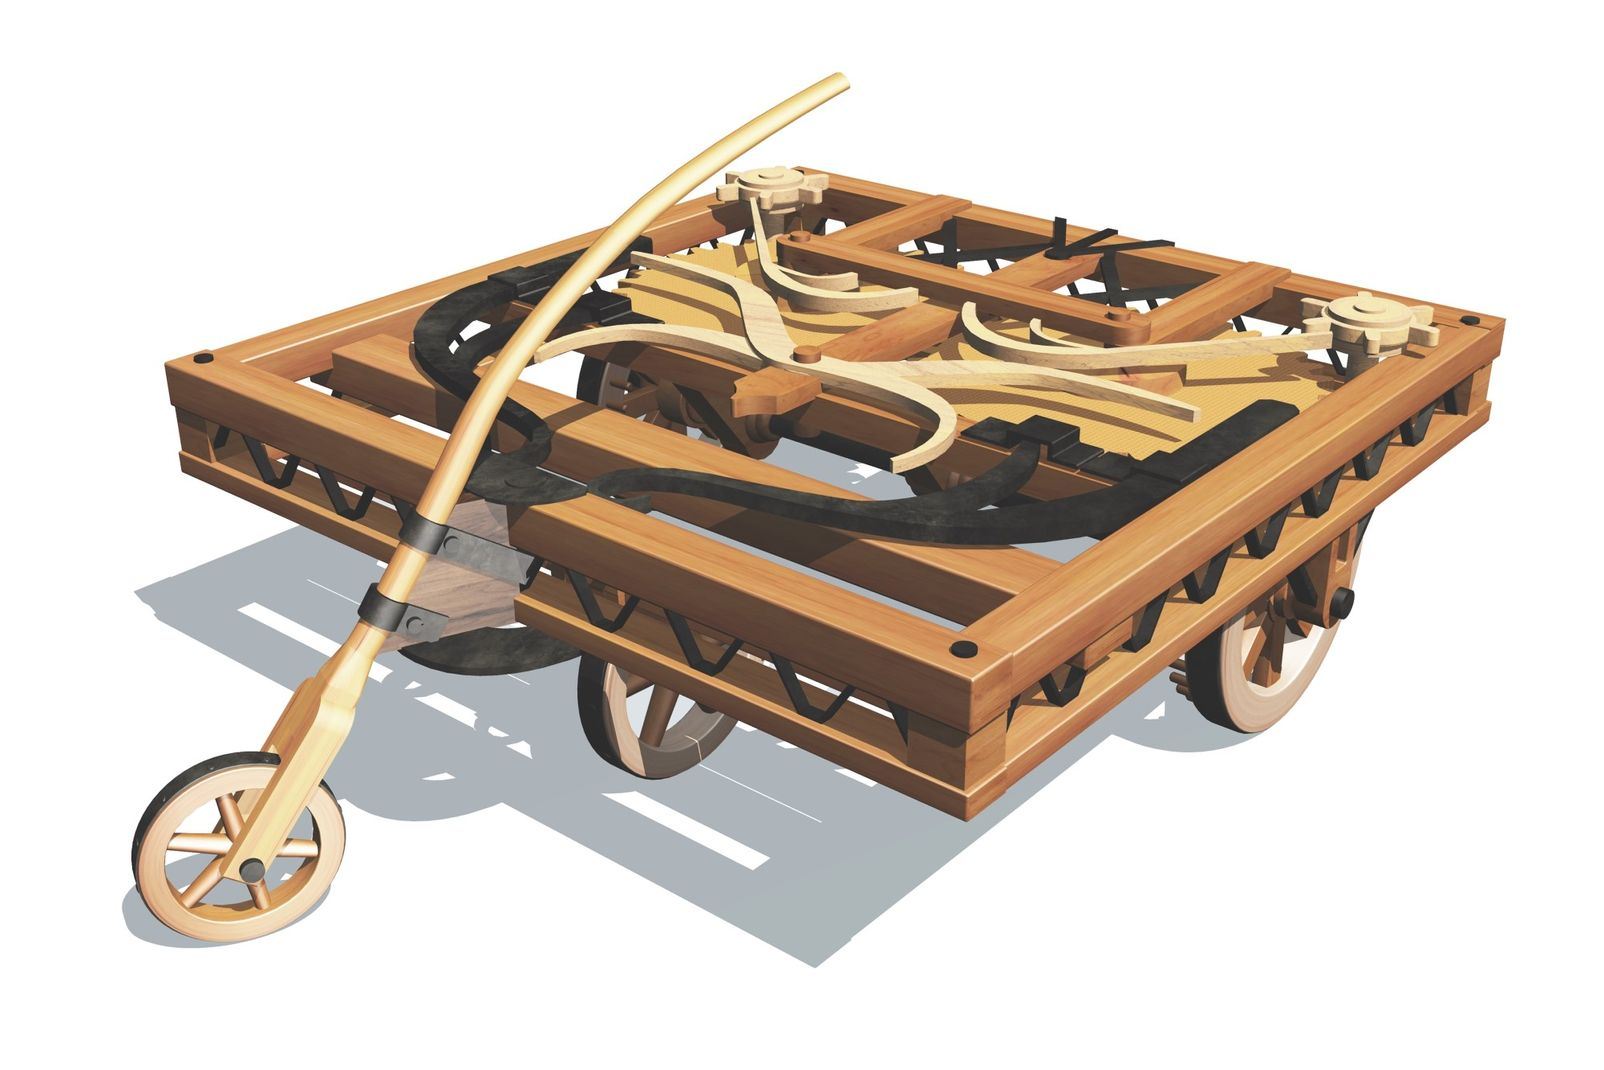
\includegraphics[width=0.35\textwidth]{ch1/figs/Vinci_car.jpg}
\caption{Model of autonomous car designed by Leonardo Da Vinci}
\label{fig:davinci_car}
\end{figure}
As we approach the Fifth Industrial Revolution (5IR), the focus shifts to a symbiotic relationship between humans and AI-powered robots, emphasizing workplace efficiency while maintaining a human-centric approach \cite{Samuels2023}. Augmented Reality (AR) plays a crucial role in this evolution, bridging the gap between humans and machines in areas such as manufacturing, healthcare, and human-robot interaction (HRI) \cite{Dalle2021}.

In the context of autonomous systems, fiducial markers (e.g., ARToolKit, AprilTags, ArUco) have become integral to robotics and AR applications. These markers facilitate robot navigation, environmental mapping, and interaction zone definition. The choice of marker system depends on specific application requirements, available computational resources, and desired accuracy.

The integration of AR and fiducial markers in robotics enhances perception, navigation, and interaction capabilities, pushing the boundaries of human-robot collaboration and making autonomous robots more adaptable and intelligent.





%@@@@@@@@@@@@@@@@@@@@@@@@@@@@@@@@@@@@@@@@@@@@@@@@@@@@@@@@@@@@@@@@@@@@@@@@@@@@@@@@@@@@@@@@@@@@@@@@@@@@@@
\section{\label{sec:probdesc}Problem Description}

As robots continue to evolve with so does our demand for more intuitive and seamless interaction with these robots. Traditional control methods often fall short when it comes to offering the flexibility and situational awareness needed to integrate robots effectively into dynamic, real-world environments. This project addresses several key challenges in the domain of mobile robot control and environmental interaction:

\begin{enumerate}
    \item \textbf{Limited Contextual Awareness}: Current remote-controlled robots often operate with minimal understanding of their surroundings, leading to inefficient navigation and potential safety hazards in complex environments.
    \item \textbf{Inflexible Control Mechanisms}: Many existing robot control systems rely on fixed command sets that do not adapt to changing environmental conditions or task requirements, limiting their versatility and usability.
    \item \textbf{Lack of Intuitive Feedback}: Users often struggle to interpret the robot's status, intentions, or responses to environmental stimuli, creating a communication gap between the human operator and the robotic system.
    \item \textbf{Absence of Dynamic Task Assignment}: Most mobile robots are pre-programmed for specific tasks and lack the ability to receive and interpret new instructions or environmental cues on the fly.
    \item \textbf{Integration Challenges}: Incorporating augmented reality (AR) elements into robotic systems presents technical challenges in terms of real-time processing, accurate marker detection, and seamless information overlay.
\end{enumerate}


%@@@@@@@@@@@@@@@@@@@@@@@@@@@@@@@@@@@@@@@@@@@@@@@@@@@@@@@@@@@@@@@@@@@@@@@@@@@@@@@@@@@@@@@@@@@@@@@@@@@@@@
%\section{\label{sec:focus}Focus}

%@@@@@@@@@@@@@@@@@@@@@@@@@@@@@@@@@@@@@@@@@@@@@@@@@@@@@@@@@@@@@@@@@@@@@@@@@@@@@@@@@@@@@@@@@@@@@@@@@@@@@@
\section{\label{sec:objectives}Objectives}

The primary objective of this project is to enhance human-robot interaction (HRI) by integrating Augmented Reality (AR) technology with mobile robotics. Leveraging AR and visual markers like ArUco codes, the robot will be able to navigate and perform tasks in a more interactive, intuitive, and human-centered manner, thus improving the overall user experience. This project focuses on providing the human operator with an augmented view of the environment and enhancing the robot’s context-awareness to better perform dynamic, real-time tasks.

More specifically, the project seeks to develop a control system that facilitates dynamic, visual-based communication between a human user and the robot. By augmenting the environment with visual markers and AR interfaces, the robot will better understand its surroundings and perform context-aware tasks. Different "control zones" will trigger specific robot behaviors based on the visual markers detected by its camera, providing real-time feedback through AR-enhanced visualizations.

\subsection{Main Objectives}
\begin{enumerate}
    \item \textbf{Development of Control Zones}: AR-based control zones will guide the robot’s behavior. These zones will define parameters such as speed adjustments, task initiation, and areas where the robot must stop or change direction based on AR markers.
    \item \textbf{Integration of Dynamic Instructions}: Using ArUco markers, the robot will receive real-time commands to perform various tasks, including navigation, task execution, and environment-specific instructions triggered by marker detection.
    \item \textbf{Environmental Mapping and Task Interaction}: The robot will use visual markers to create a simple map of its surroundings, enabling it to track landmarks, avoid obstacles, and interact with specific objects in its environment.
    \item \textbf{Improving User Engagement}: AR technology will allow users to visually instruct and monitor the robot’s progress in real-time, offering a more interactive and immersive user experience that enhances both usability and functionality.
\end{enumerate}

\subsection{Secondary Objectives}

In addition to the main objectives, the project will explore two secondary automated functionalities to improve robot autonomy:
\begin{enumerate}
    \item \textbf{Object Avoidance}: The robot will recognize specific markers (e.g., a warning cone) and avoid coming within a defined distance (e.g., 20cm) of those objects. This feature will prevent the robot from advancing if it is too close to an obstacle, even if the human operator continues pressing forward.
    \item \textbf{Wheel Slip Detection}: The robot will detect terrain changes that could cause wheel slip, such as transitioning from solid ground to a slippery surface. Instead of relying on wheel rotation counters, the robot will monitor power draw characteristics to detect traction issues and adjust accordingly.
\end{enumerate}


These enhancements aim to address the current limitations in HRI by making robot control more intuitive and responsive in dynamic environments. They also contribute to the broader goal of improving human-robot collaboration in both industrial and everyday contexts, creating a seamless and human-centered interaction model.


\section{\label{sec:terms}Terms of Reference}

This project aims to enhance human-robot interaction (HRI) by integrating Augmented Reality (AR) into a mobile robot. The system requirements, established through research, discussions with the supervisor, and analysis of the intended user environment, guide both the technical implementation and user experience. Key requirements include operating in AR-defined control zones, integrating dynamic instructions based on ArUco marker detection, environmental mapping using visual markers, providing real-time visual feedback, implementing object avoidance functionality, and detecting wheel slip events.

To meet these requirements, the system will implement several functionalities, including AR-based control zones, real-time ArUco marker processing, visual marker-based environmental mapping and obstacle avoidance, AR-based visual feedback for operators, object avoidance behavior, and wheel slip detection. Testing procedures have been outlined to ensure the system meets these requirements and functionalities, with specific sub-tests designed to check each function and requirement individually.

%\section{\label{sec:methology_overview}Methodology Overview}

\section{\label{sec:scope}Scope and Limitations}

This project was conducted under several significant constraints that shaped the scope of the research and development process. These constraints were primarily due to limitations in time, budget, and available resources, which directly impacted the scale of the implementation and the range of features that could be developed.

The project had a total budget of R2000, which restricted the procurement of high-end components and forced the use of readily available, cost-effective hardware. Additionally, the project timeline was set at three months, limiting the ability to explore more advanced functionalities and requiring a focused approach to key objectives. These constraints influenced both the design and testing phases of the project.

Furthermore, ethical considerations were taken into account, particularly in ensuring that no invasive or harmful testing methods were used. The project did not involve human or animal subjects, which helped to avoid potential ethical conflicts and the need for additional approvals.

\begin{itemize}
    \item \textbf{Time constraints:} The project had a strict timeline of three months, which limited the scope of research, prototyping, and testing phases. This required prioritizing key functionalities over more exploratory objectives.
    \item \textbf{Budget limitations:} With a budget of R2000, cost-effective hardware and software solutions had to be utilized, which influenced decisions on components such as sensors, markers, and AR technology. High-end equipment was not feasible.
    \item \textbf{Technical scope:} The project focused on AR integration for basic control and task interaction but did not include advanced machine learning algorithms or high-level autonomy features due to time and resource constraints.
    \item \textbf{Ethical limitations:} The project did not involve any human or animal subjects, thereby avoiding potential ethical conflicts. All testing was performed in controlled environments using non-invasive methods.
    \item \textbf{Environmental considerations:} The robot was tested in a limited set of predefined environments due to time and budget constraints. Broader testing in varying environments or larger spaces was outside the scope of this project.
\end{itemize}

Despite these limitations, the project successfully demonstrated the integration of AR in human-robot interaction. While the constraints limited the full realization of more advanced features, the focused approach allowed the core objectives to be met within the available resources and timeline. Further development could build upon this foundation to explore more complex functionalities and broader applications.


\section{\label{sec:plan_of_development}Plan of Development}

This thesis is structured into six chapters, each focusing on different aspects of the research and development process. The chapters build upon each other to present a coherent narrative from the conceptual framework to the implementation, testing, and conclusions of the project.

\textbf{Chapter 2: Literature Review}

Chapter 2 discusses the foundational technologies, theories, and techniques that underpin this project. It provides an overview of the state of the art in human-robot interaction (HRI), mobile robotics, and the use of Augmented Reality (AR) in robotics. This chapter will also review key research papers and methodologies that are relevant to the design and implementation of AR-enhanced control systems.

\textbf{Chapter 3: Methodology}

Chapter 3 presents the research methodology used for this project. It provides detailed explanations of the procedures, experimental setups, and tools used for the development and testing of the system. In particular, the acceptance tests will be discussed, outlining how each item of functionality and requirement will be meticulously validated through controlled tests. The methodology will emphasize how these tests demonstrate the satisfaction of both functional and system requirements.

\textbf{Chapter 4: Prototype Design}

Chapter 4 focuses on the design of the system. It provides details on the hardware and software design choices, discussing how the various subsystems (e.g., AR integration, control zones, and dynamic instructions) were conceived and implemented. For a prototype-based approach, this chapter will also describe the physical setup, robot design, and any relevant architectural decisions. Visuals such as diagrams, screenshots, and code snippets will be used to illustrate key design elements.

\textbf{Chapter 5: Results and Analysis}

Chapter 5 presents the results obtained from the system tests. These results will showcase how the robot interacted with AR markers and control zones, as well as its performance in dynamic environments. Data from the acceptance tests will be analyzed to assess the system’s functionality and its success in meeting the project’s objectives. This chapter will also include observations on the system's performance, its limitations, and any issues encountered during testing.

\textbf{Chapter 6: Discussion and Conclusion}

Chapter 6 concludes the thesis by reflecting on the overall project, summarizing the key findings, and discussing the implications of the results. It will cover the challenges faced during the project, how they were addressed, and potential areas for improvement. This chapter will also discuss future work, proposing possible enhancements and directions for further research to extend the project’s scope and applications.

\textbf{References}

Finally, all cited works, including books, journal articles, conference papers, and other relevant sources, will be compiled in the References section according to the appropriate referencing style.



%@@@@@@@ Chapter 2 - Literature Review @@@@@@@@@@@@@@@@@@@@@@@@@@@@@@@@@@@@@@@@@@
\chapter{\label{ch:lit_review} Literature Review}

This literature review provides a comprehensive exploration of the integration of Augmented Reality (AR) with mobile robotics, focusing on its applications in Human-Robot Interaction (HRI). The review is structured to cover several key areas that are crucial to the development of an AR framework for a 4WD robotic car. Here's an overview of what readers can expect to find in this literature review:

\begin{figure}[ht]
    \centering
    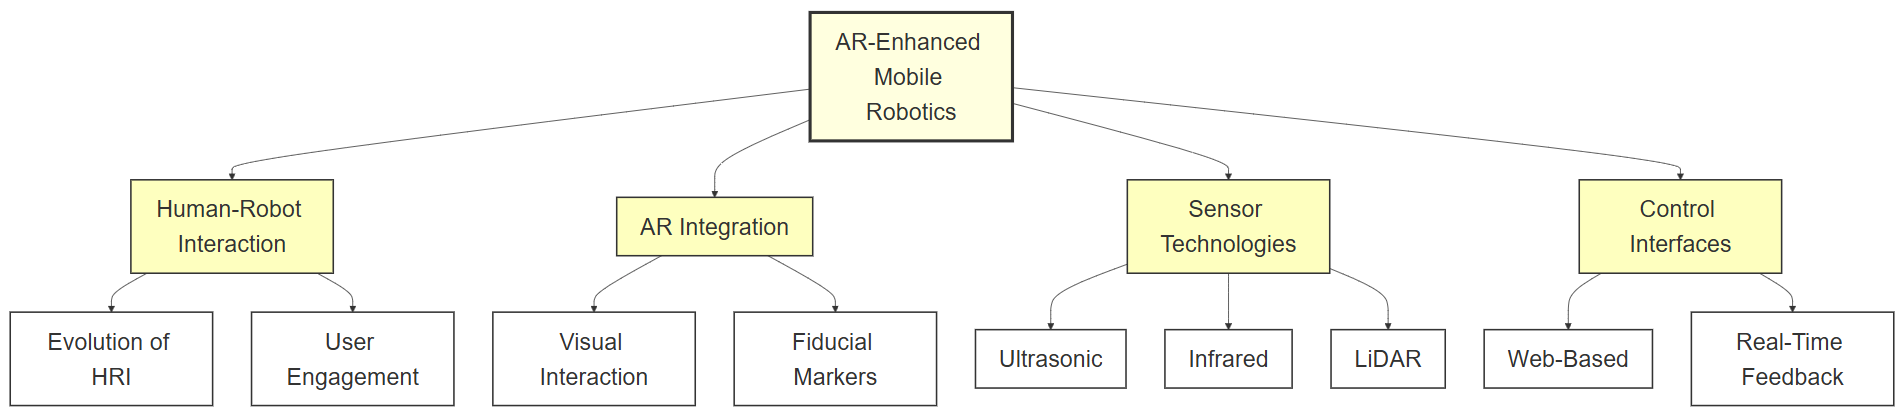
\includegraphics[width=1\textwidth]{ch2/figs/lit_overview.png}
    \caption{Overview of the structure of the literature review}
    \label{fig:Lit_overview}
\end{figure}

\section{Introduction to Human-Robot Interaction (HRI) and Augmented Reality (AR)}

Human-Robot Interaction (HRI) has seen substantial growth in both research and industrial applications, particularly with the advent of collaborative robots (cobots) that work alongside humans in dynamic environments. These robots, unlike their predecessors, are designed to safely interact with humans in shared workspaces, marking a significant shift in industrial automation. 

According to \cite{Hentout2019}, HRI evolved from isolated robot systems in manufacturing to collaborative systems where robots assist humans in complex tasks. This shift is largely due to advancements in sensing, control, and human-machine interface technologies that allow robots to perceive their environment and interact intelligently.

\begin{figure}[ht]
    \centering
    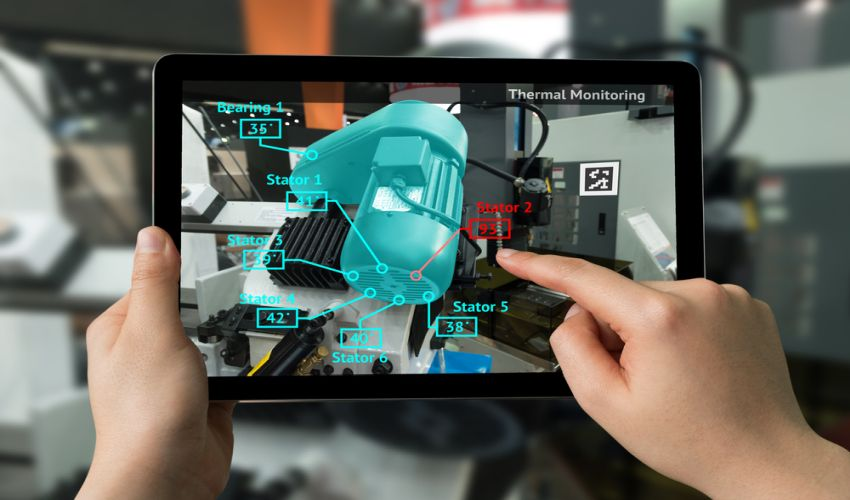
\includegraphics[width=0.5\textwidth]{ch2/figs/image_overlay.png}
    \caption{Screen Display of work environment with AR additions}
    \label{fig:AR_work_overlay}
\end{figure}

Augmented Reality (AR) has emerged as a powerful tool in enhancing HRI by providing a more intuitive and efficient way for humans to interact with robots. AR serves as a bridge that overlays digital information onto the physical environment, enabling users to better understand the robot’s actions and the task at hand \cite{Suzuki2022}. 

\subsection{Virtual Reality in Human-Robot Interaction: A Comparison with Augmented Reality}

Virtual Reality (VR) and Augmented Reality (AR) have both played significant roles in advancing Human-Robot Interaction (HRI). However, their applications and interaction paradigms differ significantly. Understanding these differences is essential when analyzing how each technology enhances the interaction between humans and robots.

VR offers a fully immersive experience where users interact with robots in a completely simulated world. This makes it particularly effective for applications such as robotic training, simulation, and remote teleoperation. For instance, VR is widely used for training operators and robots in new tasks in a risk-free virtual environment \cite{Coronado2023}. By immersing the user in a fully virtual environment, VR allows for complex robot interactions, including simulated task execution and environment navigation, which is especially useful in fields such as disaster response, industrial automation, and surgical simulations \cite{Gul2022}.

AR, on the other hand, overlays digital information onto the real world, making it more suitable for real-time, operational tasks involving physical robots. AR enables users to view critical information such as navigational data, sensor outputs, or planned robot trajectories without losing connection to their real-world environment \cite{García2019}. This makes AR ideal for applications where humans and robots share the same workspace, such as collaborative manufacturing, logistics, and maintenance tasks.

While both technologies are beneficial, this literature review will primarily focus on Augmented Reality due to its practical applications in human-robot collaboration. 

\subsection{Augmented Reality as a Tool in HRI}

AR enhances communication between humans and robots by offering real-time visualizations and feedback, thus improving situational awareness and reducing errors in task execution. Suzuki et al. \cite{Suzuki2022} propose a taxonomy of AR-enhanced HRI, highlighting the key areas where AR plays a role, such as task guidance, real-time interaction, and environment mapping. In particular, AR’s ability to provide visual feedback significantly enhances the user experience by making robot operations more transparent and reducing cognitive load.

Moreover, AR facilitates dynamic task interaction by enabling users to provide real-time instructions to the robot. This is particularly beneficial in industrial applications where task conditions change frequently. AR not only improves task accuracy but also contributes to a more efficient workflow, as robots can quickly adjust their behavior based on user commands and visual markers such as ArUco codes \cite{Suzuki2022}.

AR's applications in HRI span various industries, from manufacturing to healthcare. In manufacturing, AR has been utilized to guide robot operations through real-time visual overlays, improving precision and safety in tasks that require close human-robot collaboration \cite{Hentout2019}. Similarly, in healthcare, AR assists medical robots in performing delicate procedures by providing real-time feedback and guidance, enhancing both safety and operational efficiency \cite{Suzuki2022}. 

\section{Mobile Robotics and AR Integration}

The integration of Augmented Reality (AR) in mobile robotics has transformed how robots communicate their intentions and interact with their environment. AR not only enhances human-robot collaboration but also provides an intuitive interface for users to understand robot behavior in dynamic and complex environments. Several key studies have explored the use of AR to improve robot navigation, task execution, and real-time interaction between humans and robots.

\subsection{AR as a Communication Tool in Mobile Robotics}

One of the primary challenges in human-robot interaction is communicating the robot’s intended actions to human operators. Spatial Augmented Reality (SAR) has proven to be an effective method for achieving this. In the study by Green et al. \cite{Green2019}, SAR is used to project information about the robot’s intended movement directly onto the physical environment. This method allows users to better anticipate and respond to the robot’s actions, reducing uncertainty and enhancing collaboration. Michalos et al. \cite{Michalos2022} demonstrated the application of AR in industrial settings, where visual feedback aids in task coordination between humans and robots, leading to improved task accuracy and faster response times.

Additionally, Coovert et al. \cite{Coovert2014} explored how spatial AR techniques can improve communication between robots and humans. In their experiment, a robot used visual projections of arrows and simplified maps on the floor to indicate its short-, mid-, and long-term movement intentions. The study found that participants were able to predict the robot’s movements with high confidence when the robot projected its intended path. This is especially useful in environments where humans and robots share a workspace, such as hospitals, museums, and factories.

\begin{figure}[ht]
    \centering
    \begin{subfigure}[b]{0.4\textwidth}
        \centering
        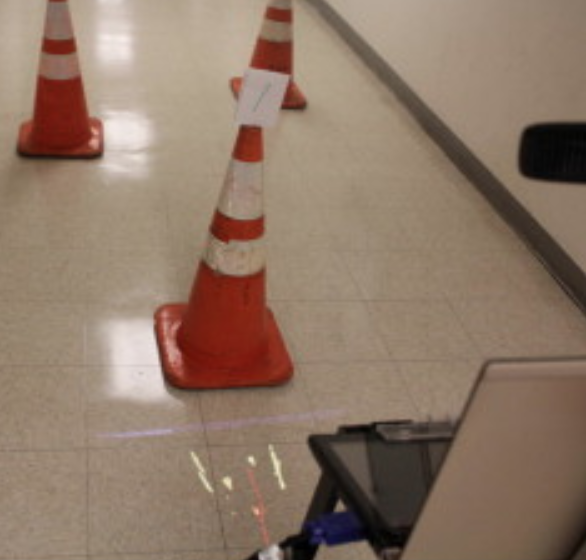
\includegraphics[width=\textwidth]{ch2/figs/robot_nav2.png}
        \caption{Robot estimating its intended movement. \cite{Coovert2014}.}
        \label{fig:estimating_path}
    \end{subfigure}
    \hspace{0.05\textwidth} % Adjust the space between the images as needed
    \begin{subfigure}[b]{0.32\textwidth}
        \centering
        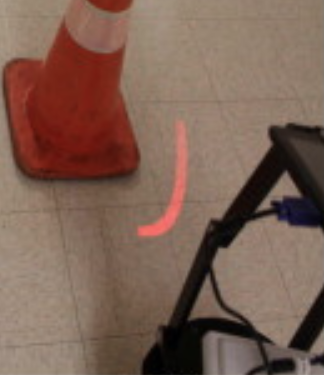
\includegraphics[width=\textwidth]{ch2/figs/robot_nav_1.png}
        \caption{Robot estimating its intended movement using AR arrows \cite{Coovert2014}.}
        \label{fig:intended_path}
    \end{subfigure}
\end{figure}



\subsection{Multimodal AR Interfaces for Human-Robot Interaction}

In addition to visual feedback, multimodal interfaces that combine AR with other modalities, such as voice or gesture recognition, have further improved human-robot interaction. Green et al. \cite{Green2019} developed a multimodal AR interface for mobile robots, allowing users to interact with the robot through visual overlays, voice commands, and gesture-based inputs. This interface improved the efficiency and accuracy of task execution in collaborative environments. The study demonstrated that multimodal AR interfaces allow for more flexible and adaptive human-robot communication, making the interaction process more intuitive and reducing cognitive load on the user.

\subsection{Applications of AR in Mobile Robotics}

AR’s integration into mobile robotics is particularly useful in environments that require constant adaptation, such as manufacturing or logistics. Michalos et al. \cite{Michalos2022} applied AR in human-robot cooperation in industrial settings, where robots must adapt to rapidly changing conditions. AR provided real-time feedback to users, helping them coordinate with robots for tasks such as assembly or quality control. Moreover, AR visualizations helped robots better navigate dynamic environments, improving both safety and efficiency.

Furthermore, AR’s ability to create real-time visual overlays in the robot’s workspace has significant implications for task planning and execution. In particular, SAR-based interfaces allow users to visually instruct robots by marking control zones or highlighting obstacles, which the robot then interprets for navigation and task completion \cite{Coovert2014}.

\subsection{Challenges and Future Directions}

While AR’s role in mobile robotics has demonstrated significant potential, challenges remain in real-time processing, accurate object recognition, and user feedback latency. As Michalos et al. \cite{Michalos2022} noted, the integration of AR into robotic systems requires further advancements in sensor technology and computational power to ensure real-time responsiveness in dynamic environments. Future research will likely focus on improving AR’s scalability in complex settings, refining multimodal interfaces, and enhancing the autonomy of mobile robots to handle more sophisticated tasks.



\section{Fiducial Marker Systems in HRI}

Augmented Reality (AR) is increasingly used in robotics to facilitate various types of Human-Robot Interactions (HRI). While multiple interaction modalities have been discussed, the remainder of this literature review will focus specifically on visual and marker-based interactions. Below is a list of the different types of interactions possible with AR:

\begin{itemize}
    \item \textbf{Visual Interaction}: AR overlays visual cues such as control zones, instructions, and real-time status feedback, enhancing human comprehension of the robot's operational environment.
    \item \textbf{Gesture-Based Interaction}: Human gestures can be interpreted by robots through AR-enhanced vision systems, reducing reliance on manual interfaces.
    \item \textbf{Speech and Command Interaction}: AR, combined with voice recognition, allows users to issue commands to robots with visual aids providing additional context.
    \item \textbf{Fiducial Marker-Based Interaction}: Fiducial markers such as ArUco or AprilTags provide robots with a way to interpret their environment, helping with localization, navigation, and object detection.
\end{itemize}

\subsection{Fiducial Marker Systems Overview}

In AR-enhanced HRI, fiducial marker systems are essential for real-time contextual interactions. These systems use visually distinct markers that robots detect through cameras. The most commonly used marker systems include ARToolKit, AprilTags, and ArUco markers, each with unique characteristics suited to various applications.
\begin{figure}[ht]
    \centering
    \begin{subfigure}[b]{0.25\textwidth}
        \centering
        
\includegraphics[width=\textwidth]{ch1/figs/ARToolkit.jpg}
        \caption{ARToolKit}
        \label{fig:artoolkit}
    \end{subfigure}
    \hfill
    \begin{subfigure}[b]{0.25\textwidth}
        \centering
        
\includegraphics[width=\textwidth]{ch1/figs/AprilTag.png}
        \caption{AprilTags}
        \label{fig:apriltags}
    \end{subfigure}
    \hfill
    \begin{subfigure}[b]{0.25\textwidth}
        \centering
        
\includegraphics[width=\textwidth]{ch1/figs/ArUco.png}
        \caption{ArUco markers}
        \label{fig:aruco}
    \end{subfigure}
    \caption{Visual comparison of different marker systems}
    \label{fig:markers}
\end{figure}

\textbf{ARToolKit} is one of the earliest fiducial marker systems developed for augmented reality applications. It was widely adopted in early AR systems due to its simplicity and moderate computational requirements. In HRI, ARToolKit has been used in early experiments involving robot navigation and control. However, its robustness is limited compared to more modern systems, and it struggles under challenging lighting conditions \cite{Suzuki2022}.

\textbf{AprilTags} are an improvement over ARToolKit, offering significantly higher robustness and detection accuracy. As \cite{Daponte2020} highlights, AprilTags are designed to provide accurate detection even in adverse environments with variable lighting and occlusion. AprilTags have been extensively used in industrial applications where precise localization is critical, such as warehouse automation and autonomous guided vehicles (AGVs). The system is computationally heavier than ARToolKit but provides superior reliability, making it suitable for applications that demand accuracy over speed \cite{Filus2023}.

\textbf{ArUco markers} are designed with computational efficiency in mind, offering high detection speed without sacrificing much in terms of accuracy. This makes them ideal for real-time applications, particularly in mobile robotics where swift responses are critical. \cite{Husar2022} notes that ArUco markers have been used in various applications including navigation and task execution in dynamic environments such as warehouses. Their simplicity and widespread software support make them a popular choice for developers working on real-time robotic systems.

\begin{table}[h]
\centering
\caption{Comparison of Fiducial Marker Systems}
\resizebox{\textwidth}{!}{
\begin{tabular}{|p{3cm}|p{2cm}|p{2cm}|p{4cm}|p{4cm}|}
\hline
\textbf{Marker System} & \textbf{Robustness} & \textbf{Detection Accuracy} & \textbf{Computational Efficiency} & \textbf{Applications} \\
\hline
ARToolKit     & Moderate    & Good      & Moderate      & Early AR applications \\
AprilTags     & High        & Excellent & Moderate-High & Robotics \\
ArUco Markers & High        & Good      & High          & Real-time robot navigation \\
\hline
\end{tabular}
}
\end{table}


\subsection{Choosing the Best Marker System for the Project}

Given the requirements of the project, which involve real-time processing, dynamic navigation, and user interaction, ArUco markers are the most suitable choice. As \cite{Filus2023} demonstrates, ArUco markers provide a good balance between computational efficiency and detection accuracy, making them ideal for mobile robotic systems that require fast decision-making. Additionally, the ease of integration with commonly used robotics software such as ROS (Robot Operating System) further justifies their selection for this project.

\subsection{Visual Interaction in AR-Enhanced HRI}

Visual interaction is one of the most common and effective forms of interaction in Augmented Reality (AR)-enhanced Human-Robot Interaction (HRI). It enables users to interact with robots by visualizing contextual information directly within their physical environment. This can include task instructions, control zones, and real-time feedback on the robot's status and performance.

In AR-enhanced visual interaction, the robot's actions and intentions are augmented with overlays that help the human user make informed decisions during interaction. \cite{Suzuki2022} provides a comprehensive overview of how visual interaction enhances HRI by improving situational awareness and reducing the complexity of controlling robotic systems. This is especially useful in industrial applications, where workers interact with robots to execute precise tasks, such as assembly and quality control.

\subsubsection{Applications of Visual Interaction}

Visual interaction in AR has broad applicability across various fields, with significant benefits in improving task accuracy, communication, and overall efficiency. Some notable applications include:
\begin{itemize}
    \item \textbf{Manufacturing and Assembly}: In industries such as automotive and aerospace, visual interaction is used to overlay task instructions on the assembly line, helping workers follow complex procedures. This reduces human error and increases productivity by providing step-by-step visual guidance \cite{Daponte2020}.
    \item \textbf{Healthcare}: In robotic surgery and rehabilitation, visual interaction allows surgeons and therapists to see real-time data overlaid on patients, enhancing precision and safety. AR enhances the accuracy of procedures by showing virtual boundaries and guidelines, ensuring that robots move correctly within the workspace \cite{Husar2022}.
    \item \textbf{Warehouse and Logistics}: In logistics and warehouse management, AR systems provide real-time visual cues to workers handling robotic systems for item sorting, picking, and delivery. \cite{Husar2022} explores the use of AR to improve warehouse efficiency by overlaying instructions on specific zones, helping workers interact more intuitively with robotic arms and autonomous guided vehicles (AGVs).
\end{itemize}

\subsubsection{Visual Feedback and Real-Time Interaction}

One of the most significant advantages of AR-enhanced visual interaction is the provision of real-time feedback, which facilitates more intuitive robot control. \cite{Filus2023} investigates the real-time testing of vision-based systems in AGVs using ArUco markers and AR visualizations. Their research highlights how visual feedback improves decision-making in dynamic environments, helping robots navigate autonomously with greater efficiency.

Visual feedback can take various forms:
\begin{itemize}
    \item \textbf{Control Zones}: Specific areas within the robot's environment are highlighted using AR, guiding the robot's actions and helping the user visualize where the robot can move or interact with objects.
    \item \textbf{Status Updates}: Information such as battery levels, current tasks, or environmental hazards can be projected onto the robot’s workspace, allowing users to quickly assess and adjust the robot’s behavior as needed.
    \item \textbf{Error Detection}: AR systems can visually highlight potential errors in the robot's movements, such as collisions, off-course navigation or wheel slipping, enabling quick corrective actions.
\end{itemize}


Suzuki et al. \cite{Suzuki2022} emphasizes that visual interaction not only enhances HRI but also promotes collaboration between human operators and robots by reducing cognitive load. By providing real-time visual cues, AR improves situational awareness and makes controlling robots more intuitive, particularly in environments where precision is critical.

However, there are certain limitations. \cite{Daponte2020} discusses the challenges of accurately overlaying visual data in real-time, particularly in environments with inconsistent lighting, reflections, or occlusions. Additionally, the processing demands of rendering real-time visualizations may limit the performance of systems with constrained computational resources.

\section{AR's Role in Improving User Engagement}

Augmented Reality (AR) has significantly enhanced user engagement with robotic systems, particularly in Automated Guided Vehicles (AGVs). By providing intuitive visual feedback and real-time streaming data, AR improves both the psychological and practical interaction between humans and AGVs. The combination of augmented reality and robotics has been a topic of significant research interest, as AR makes robots more intuitive to control and increases user trust in automated systems.

\subsection{Enhancing User Engagement through Real-Time Feedback and Visualization}

One of the key strengths of AR is its ability to provide real-time feedback and visualizations, allowing users to intuitively understand the robot’s actions and status. AR-infused streaming technology improves human-robot collaboration by projecting real-time data, control zones, and navigation paths onto the robot's environment \cite{Fu2023}. This continuous stream of real-time data reduces cognitive load, enabling users to anticipate and control AGV movements more effectively in dynamic environments. Such real-time visualization allows users to engage more deeply with robotic systems, increasing their confidence in controlling AGVs.

In particular, \cite{Fu2023} explore how AR is utilized across different robotic applications, including medical, industrial, and social robotics. For AGVs, they highlight AR's capability to enhance human-robot collaboration by improving real-time task allocation and decision-making processes. The visual feedback offered by AR systems reduces the need for constant manual adjustments, thereby increasing operator efficiency \cite{Fu2023}.

In industrial scenarios, \cite{Makhataeva2020} emphasize the role of AR in improving user engagement through its intuitive interfaces. They note that AR helps operators visualize tasks more clearly, thus reducing the learning curve for new users while providing advanced feedback for experienced operators. This is important in environments where quick decisions are necessary \cite{Makhataeva2020}.

\subsection{Psychological and Practical Benefits}

The psychological impact of AR on user engagement is considerable. Real-time visualizations, such as path projections or task instructions, create a more predictable and transparent interaction between humans and robots. Users become more confident when they can clearly see an AGV's next move, which reduces uncertainty about the robot's behavior and enhances user trust. This \textbf{increased predictability} improves user satisfaction and promotes wider adoption of AR-enabled robotic systems \cite{Coovert2014}.

AR also offers practical benefits in rehabilitation settings, where users can engage with robotic systems in therapy. As Makhataeva \cite{Makhataeva2020} points out, AR interfaces allow users to interact with AGVs or rehabilitation robots in a natural way, improving patient recovery outcomes. The immersive nature of AR encourages patient involvement, which is crucial in therapeutic contexts \cite{Makhataeva2020}.

\section{Web-Based Control Interfaces}
Having a functional robot is all well and good but if the robot has an unpleasant or inefficient interface then it ruins the whole user experience. This section will detail different methods of implementing web-based control interfaces, focusing on real-time communication, user interaction, and video streaming. 

\subsection{Webserver Framework Options}

\textbf{Flask} is a lightweight Python web framework known for its simplicity and flexibility\cite{moraneus2024}. It is particularly well-suited for the rapid development of web-based control interfaces. Flask is easy to set up and use, making it ideal for prototyping and small to medium-sized applications. It integrates well with Python libraries commonly used in robotics. However, for real-time features, additional libraries may be required, and its performance can be a concern for large-scale applications.

\textbf{Node.js} is a JavaScript runtime built on Chrome’s V8 engine, recognized for its event-driven, non-blocking I/O model. Its asynchronous nature makes it highly suitable for real-time applications \cite{asiandigitalhub2023}. Node.js also benefits from a large ecosystem of packages and libraries and is capable of efficiently handling many simultaneous connections. However, it may require more setup compared to Flask, and its callback-based programming can be complex for beginners.

\textbf{WebSocket integration} is essential for real-time control and data streaming, providing low-latency, bidirectional communication over a single TCP connection \cite{websockets}. This is particularly advantageous when sending control commands and receiving video streams. WebSockets can be integrated with both Flask and Node.js, though careful implementation is required to handle issues such as connection drops and reconnections, and additional security measures may be necessary.

\textbf{Apache and Nginx} are traditional web servers that are robust, highly scalable, and performant, making them popular choices in production environments. They offer extensive documentation and strong security features. However, they may be more complex to set up and configure, and can be overkill for smaller projects or embedded systems like Raspberry Pi \cite{jankov2019}. They are typically used in conjunction with application servers rather than for standalone dynamic content.

Flask or Node.js, combined with WebSocket integration, would likely be the most suitable choices due to their ease of use and real-time capabilities. For this project Flask will be implemented due to its ease of understanding for a beginner.

\subsection{Security and User Experience}

While security is a crucial aspect of any robotic system, especially those controlled through web-based interfaces, it's important to note that for the scope of my project, I've chosen not to delve deeply into privacy and security concerns. This decision allows me to focus more intensively on the core functionality and user experience aspects of the system.

In a real-world application, however, it would be critical to implement robust security measures. These would typically include encryption protocols like TLS (Transport Layer Security) to protect the integrity and confidentiality of data exchanged between the robot and the user interface. Additionally, strong authentication mechanisms would be necessary to prevent unauthorized access to the robot's controls.

\section{Sensor Technologies in Human-Robot Interaction}

When discussing the AR technology, it's difficult to do so without making mention of sensors, sensors allow machines to interact with their environments. Sensors are to machines what eyes and ears are to humans. This section serves as a review for the applicable sensors relevant to this project which is designing a AR framework for a 4WD robotic car.

\subsection{Ultrasonic Sensors} 
Ultrasonic sensors are a common choice in mobile robotics due to their effectiveness in obstacle avoidance and distance measurement. These sensors emit ultrasonic waves and measure the time it takes for the waves to reflect back from an object, allowing the robot to calculate the distance from obstacles \cite{maupin2023ultrasonic}. This capability provides spatial awareness that is critical for safe navigation. Below is a basic diagram showcasing the operation of an HC-SR04 Infrared Sensor.

\begin{figure}[ht]
    \centering
    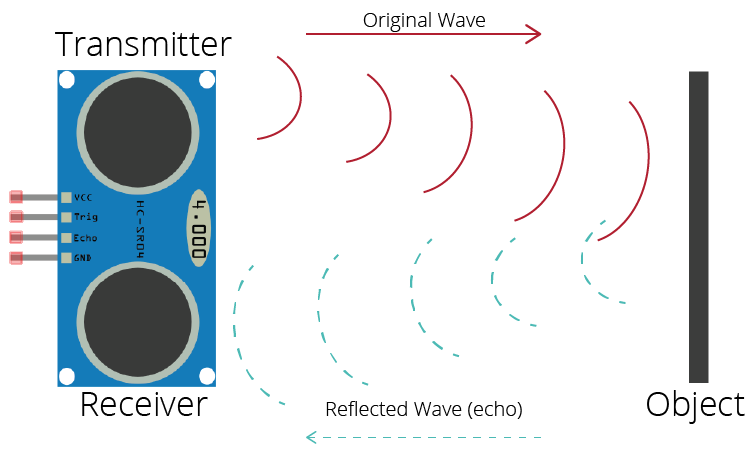
\includegraphics[width=0.53\textwidth]{ch2/figs/ultrasonic_sensor.png} % Change the path if the image is located elsewhere
    \caption{Operation of an Ultrasonic Sensor {\cite{randomnerd2021ultrasonic}}}
    \label{fig:ultrasonic_sensor}
\end{figure}

\noindent
Below is a comparison of some common ultrasonic sensors used in mobile robotics.

\begin{table}[ht]
\centering
\caption{Comparison of Ultrasonic Sensors}
\begin{tabularx}{\textwidth}{|c|c|X|c|c|c|}
\hline
\textbf{Model} & \textbf{Range (cm)} & \textbf{Operating Voltage (V)} & \textbf{Accuracy} & \textbf{Field of View} & \textbf{Size (mm)} \\ \hline
HC-SR04 & 2-400 & 5 & ±0.3 cm & 15 degrees & 45 x 20 x 15 \\ \hline
Maxbotix MB1000 & 20-645 & 2.5-5.5 & ±1\% & 42 degrees & 22 x 20 x 16 \\ \hline
Parallax PING))) & 3-300 & 5 & ±0.5 cm & 20 degrees & 22 x 46 x 16 \\ \hline
\end{tabularx}
\label{tab:ultrasonic_comparison}
\end{table}

Ultrasonic sensors are advantageous because of their simplicity, affordability, and ease of integration. For this project, they could provide an excellent mechanism for detecting nearby obstacles, which is essential for navigation in dynamic environments. Some key properties of ultrasonic sensors include:

\begin{itemize}
    \item \textbf{Wide Range of Detection}: As seen in the table, ultrasonic sensors like the HC-SR04 and Maxbotix MB1000 can detect objects at distances ranging from a few centimeters to several meters. This is beneficial for both short-range and long-range obstacle avoidance.
    \item \textbf{Accuracy and Precision}: Depending on the model, ultrasonic sensors offer good accuracy for distance measurements. For example, the Maxbotix MB1000 boasts an accuracy of ±1\%, helping ensure that the robot reacts promptly and effectively to its surroundings.
    \item \textbf{Field of View (FoV)}: The field of view differs between sensors, affecting the robot's perception. A larger FoV allows the robot to detect obstacles from a wider angle, but may result in less precise focus on individual objects.
\end{itemize}

Integrating ultrasonic sensors with augmented reality (AR) offers the possibility of visualizing sensor data in real time. For example, AR can highlight areas where the robot detects obstacles, providing the operator with enhanced spatial awareness, preventing collisions, and improving task efficiency. Additionally, real-time data streaming through a visual interface allows for immediate adjustments to the robot's behavior based on sensor readings.

\subsection{Infrared Sensors} 

Infrared (IR) sensors are commonly used in mobile robotics for tasks such as proximity detection, line-following, and object avoidance. These sensors emit infrared light and detect the reflection from nearby objects, making them effective for short-range detection in controlled environments \cite{benet2002infrared}.

While standard IR sensors, such as the basic proximity IR sensors, serve well in obstacle avoidance and object detection, they have limitations in terms of range, field of view, and accuracy. These standard sensors perform well in specific lighting conditions but struggle in environments with significant ambient light interference \cite{rhydo2024}.

\subsubsection{The Dagu Infrared Compound Eye} 
The \textbf{Dagu Infrared Compound Eye} shares basic functionality with standard IR sensors but offers significant enhancements. Unlike single-point IR sensors, the Dagu sensor features a compound array of multiple infrared detectors, allowing for a much wider field of view and multi-directional sensing. This enables the robot to detect objects from multiple angles, enhancing spatial awareness and enabling more complex navigation and object tracking tasks \cite{rhydo2024}.

Integrating the \textbf{Dagu Infrared Compound Eye} into this project would extend the robot's capabilities by improving its obstacle detection, particularly in dynamic and complex environments. The sensor’s wide field of view, combined with real-time AR feedback, could provide users with a more intuitive control system and greater situational awareness, thereby improving human-robot interaction (HRI). Moreover, the sensor could aid in tasks requiring precise spatial awareness, such as navigating around obstacles or detecting specific objects \cite{benet2002infrared}.

\begin{table}[ht]
\centering
\caption{Specifications of the Dagu Infrared Compound Eye}
\begin{tabular}{|c|c|}
\hline
\textbf{Specification} & \textbf{Value} \\ \hline
Number of Detectors & 4 infrared sensors \\ \hline
Detection Range & 200mm \\ \hline
Operating Voltage & 5V \\ \hline
Power Consumption & 10 mA \\ \hline
\end{tabular}
\label{tab:dagu_infrared}
\end{table}


Additionally, this sensor could provide valuable data that could be visualized for the user through augmented reality (AR), enabling a more interactive and user-friendly experience.

\subsection{LiDAR Sensors} LiDAR (Light Detection and Ranging) is an essential technology for mobile robotics that uses laser light to measure distances and create 3D maps of environments. By utilizing LiDAR sensors, mobile robots can detect obstacles, map their surroundings, and navigate autonomously \cite{yang2022lidar}.

\begin{figure}[hb]
    \centering
    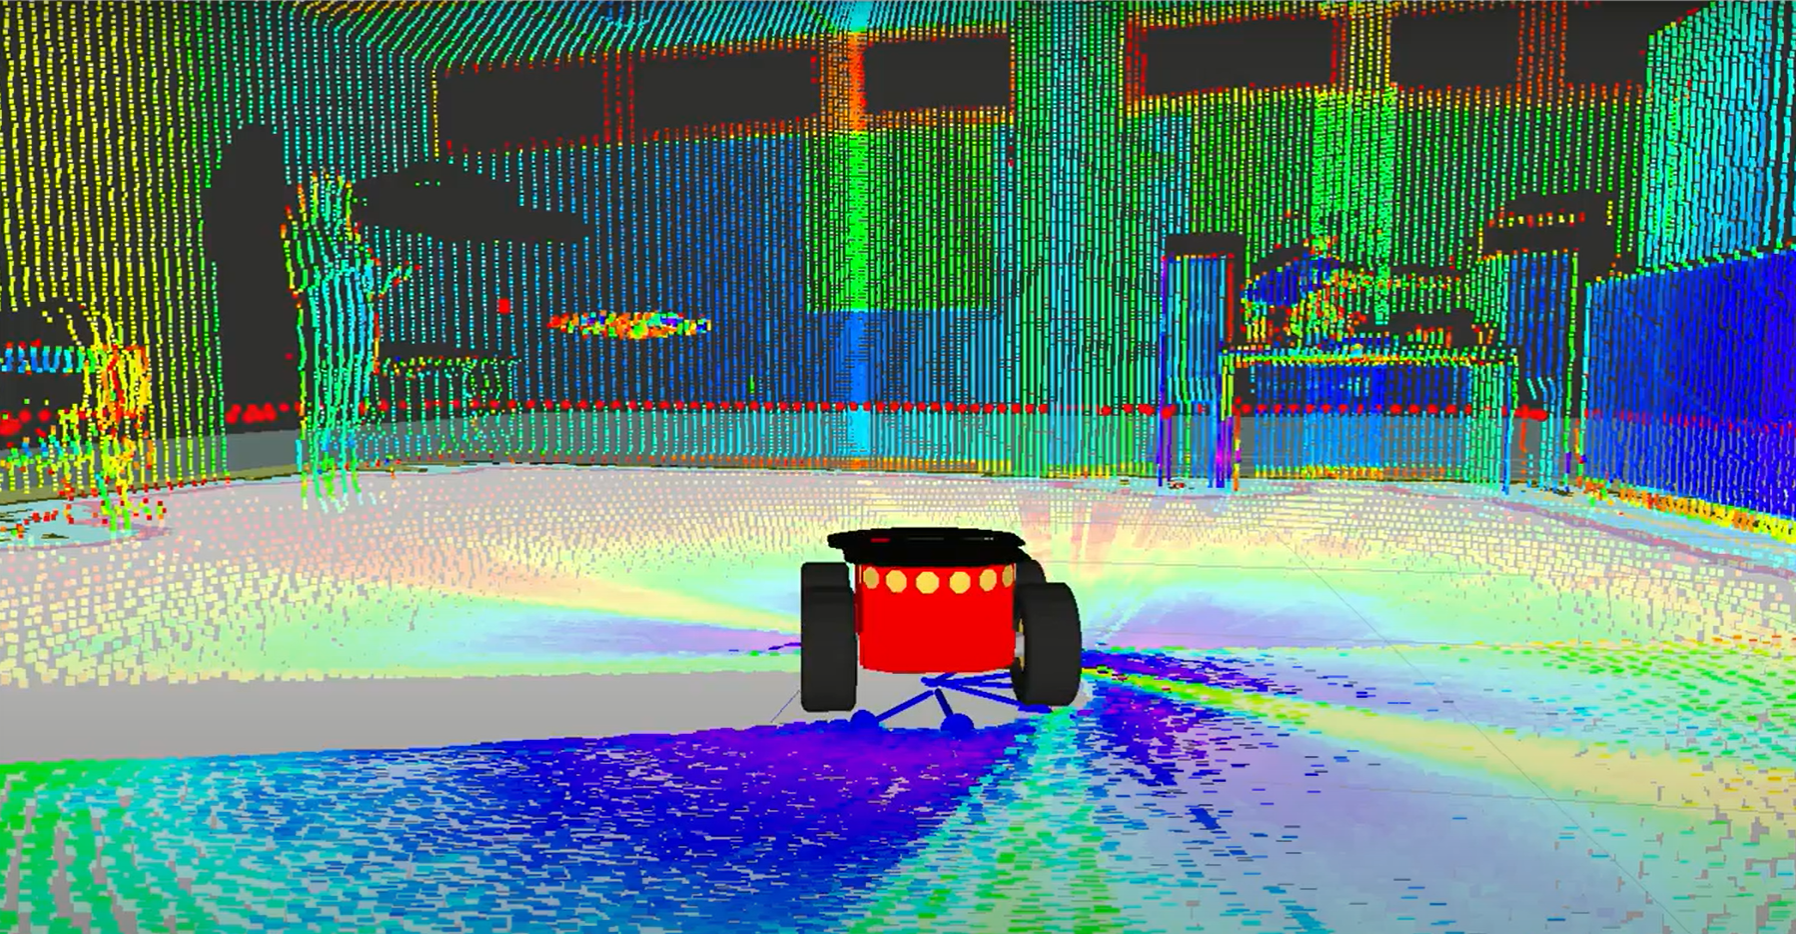
\includegraphics[width=0.5\textwidth]{ch2/figs/lidar_graphic.png}
    \caption{LiDAR scanning and mapping process in mobile robotics.}
    \label{fig:lidar_graphic}
\end{figure}

For this review, two LiDAR sensors will be considered although they will not be considered for the project itself: \textbf{RPLIDAR A1} and \textbf{TF Mini LiDAR (ToF) Laser Range Sensor V2.0}. These sensors offer capabilities that can significantly enhance the robot's ability to perceive and interact with its environment. Below is a comparison of their specifications \cite{yang2022lidar}:

The \textbf{RPLIDAR A1} is a 360-degree scanning LiDAR sensor capable of creating a comprehensive map of the robot's surroundings in real time. This would enable the robot to detect objects and obstacles from all directions, making it ideal for use in complex environments where autonomous navigation is crucial.

\begin{table}[htpb]
\centering
\caption{Comparison of RPLIDAR A1 and TF Mini LiDAR (ToF) Sensors}
\label{tab:lidar_comparison}
\begin{tabular}{|l|l|l|} 
\hline
\textbf{Specification} & \textbf{RPLIDAR A1} & \textbf{TF Mini LiDAR (ToF)}  \\ 
\hline
Max Range              & 12m                 & 12m                           \\ 
\hline
Resolution             & 0.2cm               & 1cm                           \\ 
\hline
Field of View          & 360° (horizontal)   & 3.6° (horizontal)             \\ 
\hline
Sample Rate            & 8000 samples/sec    & 1000 samples/sec              \\ 
\hline
Power Consumption      & 5V, 500mA           & 5V, 140mA                     \\ 
\hline
Interface              & UART, USB           & UART                          \\ 
\hline
Size (mm)              & 97.5 x 60 x 38      & 42 x 15 x 16                  \\
\hline
\end{tabular}
\end{table}

On the other hand, the \textbf{TF Mini LiDAR (ToF)} sensor, although more limited in its field of view, offers a compact and lightweight design, making it suitable for applications requiring focused, high-speed distance measurement. Its small size and low power consumption could be beneficial for tasks where precise distance measurements are needed without adding significant weight or power demands.

Both sensors would improve the robot's environmental mapping and obstacle detection capabilities. Visualizing the LiDAR data in an AR interface would provide real-time feedback to users, enabling them to monitor the robot’s surroundings and make informed decisions about its movement.

\section{Conclusion}

This literature review has explored the integration of Augmented Reality (AR) with mobile robotics, focusing on Human-Robot Interaction (HRI). Key areas such as fiducial marker systems like ArUco markers, sensor technologies, and web-based control interfaces were examined to assess their role in improving real-time visualization and user interaction with robots.

AR has emerged as a crucial tool in enhancing HRI, offering real-time feedback, improved situational awareness, and better task performance. Additionally, sensors such as ultrasonic and LiDAR, combined with AR, hold promise for optimizing navigation and obstacle avoidance in mobile robots.

While AR shows significant potential for advancing HRI, challenges such as real-time processing limitations and the need for secure web-based interfaces remain. These insights will guide the development of my AR framework for the 4WD robotic car, focusing on real-time visualization, intuitive control, and efficient sensor integration.


%@@@@@@@ Chapter 3 - Requirements and Specifications @@@@@@@@@@@@@@@@@@@@@@@@@@@@@@@@@@@@@@@@@@
%\chapter{\label{ch:req_and_specs} Requirements and Specifications}

This project builds on the primary objective of enhancing human-robot interaction (HRI) by integrating Augmented Reality (AR) into a mobile robot. As outlined in Section \ref{sec:objectives}, the system needs to meet specific requirements to ensure it performs as intended. These requirements were established through research, discussions with supervisor, and analysis of the intended user environment. The requirements are designed to guide both the technical implementation and the user experience, ensuring the robot operates seamlessly with AR-based control systems.

\begin{itemize}
    \item \textbf{R1.} The robot must operate in different control zones, defined by AR markers, and adjust its behavior accordingly (e.g., slowing down, stopping, or performing a task).
    \item \textbf{R2.} The system must integrate dynamic instructions based on ArUco marker detection, allowing for real-time task updates.
    \item \textbf{R3.} The robot must map its environment using visual markers and avoid obstacles based on AR feedback.
    \item \textbf{R4.} The AR interface must provide real-time visual feedback for the human operator to improve task monitoring and control.
    \item \textbf{R5.} The robot must include object avoidance functionality, ensuring it maintains a safe distance from recognized obstacles (e.g., warning cones) based on AR markers.
    \item \textbf{R6.} The system should detect and respond to wheel slip events caused by changes in surface traction, providing stability during operation.
\end{itemize}

To meet these requirements, the system will implement the following functionalities:

\begin{itemize}
    \item \textbf{F1.} Implementation of AR-based control zones that dynamically adjust robot speed, direction, or initiate tasks based on detected markers (R1).
    \item \textbf{F2.} Real-time processing of ArUco markers to update task instructions and provide context-specific navigation and task execution (R2).
    \item \textbf{F3.} The robot will use visual markers for environmental mapping and will avoid obstacles based on this feedback (R3).
    \item \textbf{F4.} AR-based visual feedback will provide the human operator with real-time monitoring of the robot’s actions and environmental interactions (R4).
    \item \textbf{F5.} Integration of object avoidance behavior, ensuring the robot maintains a safe distance from obstacles based on AR marker detection (R5).
    \item \textbf{F6.} Implementation of wheel slip detection functionality that monitors the robot's power draw to identify surface traction changes (R6).
\end{itemize}

Testing will be performed to ensure that the system meets the outlined requirements and functionalities. The table below shows the breakdown of the sub-tests to be performed, with each test linked to the specific functions and requirements it checks.

\begin{table}[ht]
\centering
\caption{Breakdown of sub-tests to be performed in the acceptance testing.}
\label{tab:testing}
\begin{tabular}{|c|p{5cm}|c|c|}
\hline
\textbf{Test Number} & \textbf{Description} & \textbf{Functions Checked} & \textbf{Requirements Tested} \\ \hline
T1                   & Test the robot’s behavior in AR-based control zones   & F1  & R1   \\ \hline
T2                   & Test real-time ArUco marker detection for dynamic instructions & F2  & R2   \\ \hline
T3                   & Test environmental mapping and obstacle avoidance based on AR markers & F3  & R3, R5 \\ \hline
T4                   & Test AR-based visual feedback for real-time monitoring & F4  & R4   \\ \hline
T5                   & Test object avoidance system using visual markers   & F5  & R5   \\ \hline
T6                   & Test wheel slip detection and response functionality & F6  & R6   \\ \hline
\end{tabular}
\end{table}




%@@@@@@@ Chapter 3 - Methodology  @@@@@@@@@@@@@@@@@@@@@@@@@@@@@@@@@@@@@@@@@@@@@@@
\chapter{\label{ch:methodology} Methodology}
This chapter details the design and implementation of a mobile robotic system using augmented reality (AR), fiducial markers, and remote monitoring to improve human-robot interaction (HRI). It builds on existing research in computer vision-based navigation, AR for HRI, and internet-controlled mobile robots. Design decisions are justified with related literature and practical system requirements
\section{\label{sec:overview} Overview}

The high-level diagram illustrates the mobile robot project's architecture, showcasing key components: Raspberry Pi (central processor), camera module, motor control system, fiducial markers, and web-based control interface. The data flow begins with the camera capturing video, which the Raspberry Pi processes for marker detection and navigation. Simultaneously, the web interface sends commands to the Raspberry Pi, which also streams video back to the user. 

\begin{figure}[H]
    \centering
    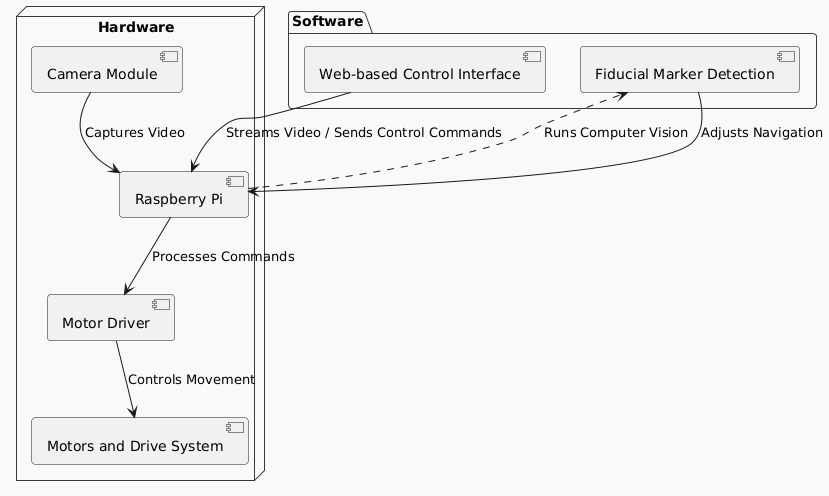
\includegraphics[width=0.7\textwidth]{ch3/figs/diagram.png}
    \caption{High Level Diagram of how the project will run}
    \label{fig:high_level_diagram}
\end{figure}

The methodology centers on the development of a mobile robot system capable of navigation, interaction, and real-time feedback, using AR markers and remote control via a Raspberry Pi board. Inspired by the works of La Delfa et al. \cite{delfa2015}, Jacobsen et al. \cite{jacobsen2018}, and Vanitha et al. \cite{vanitha2016}, this project seeks to incorporate advances in fiducial marker systems and AR interfaces to improve the efficiency and user engagement in controlling mobile robots.



%@@@@@@@ Chapter 4 - Design @@@@@@@@@@@@@@@@@@@@@@@@@@@@@@@@@@@@@@@@@@@@@@@@@@@@@
\chapter{\label{ch:ch4} Design ad Implementation}

This is the design chapter intro and explaining structure etc.

\section{\label{sec:ch4_firstsec}System Design}

This section presents the system design with nice illustrations.
\section{\label{sec:sys_architecture} System Architecture}

The project is composed of several key components, below is a high level overview of all the components that are needed in order execute the project properly.

\begin{table}[ht]
\centering
\caption{System Architecture Components}
\label{tab:system_architecture}
\begin{tabular}{|p{5cm}|p{10cm}|}
\hline
\textbf{Component} & \textbf{Description} \\ \hline
Microcontroller/Processor & Manages computer vision algorithms and interfaces with hardware. Responsible for overall system control and data processing. \\ \hline
Web Camera & Provides real-time video feed for remote monitoring and vision tasks. Captures high-quality images for processing. \\ \hline
Motor and Drive System & Four-wheel drive system for robot mobility. Includes motors and a motor controller for precise movement control.\\ \hline
Fiducial Markers & Visual markers (e.g., ArUco or AprilTag) placed in the environment to assist with localization and navigation.\\ \hline
Web-based Control Interface & Allows remote control of the robot’s movements and camera functions, with video streaming capabilities. \\ \hline
Power Supply & Provides electrical power to all components of the system. Needs to support extended operation and peak power demands. \\ \hline
Chassis & Physical structure of the robot that houses and protects all components. Designed for durability and optimal component placement.  \\ \hline
Sensors & Additional sensors for environmental awareness (e.g., ultrasonic sensors, IMU, GPS).\\  \hline
Communication Module & Enables wireless communication between the robot and the control interface, supporting long-range and reliable data transmission. \\ \hline
\end{tabular}
\end{table}


%@@@@@@@ Chapter 4 - Testing @@@@@@@@@@@@@@@@@@@@@@@@@@@@@@@@@@@@@@@@@@@@@@@@@@@@@
\chapter{Modular Testing}

The testing process for this project was conducted in a systematic and incremental manner to ensure that each subsystem functioned as expected before being integrated into the final system. The approach involved testing each module independently, followed by creating interfaces between these modules, and finally testing the interactions between them. This strategy helped identify and resolve issues early, ensuring that the final system was robust and performed as required.

\begin{figure}[H]
	\centering
	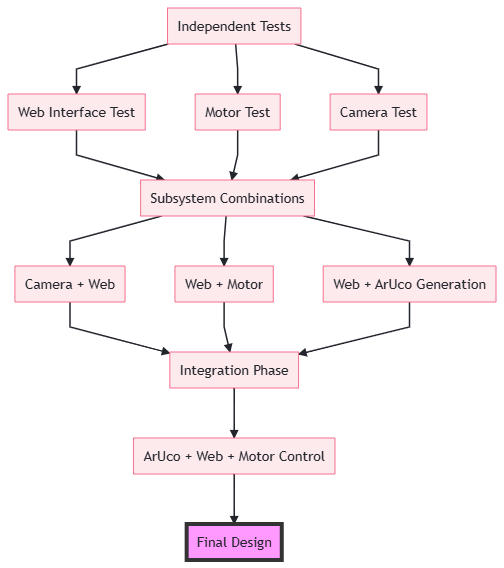
\includegraphics[width=0.7\textwidth]{Testing/figs/flow.png}
	\caption{Illustration of different levels of testing implemented in the project.}
	\label{fig:testing_levels}
\end{figure}

\section{Independent Module Testing}

Each subsystem of the robot was tested individually using Python scripts to verify functionality before integration into the full system. This modular testing allowed for focused troubleshooting and ensured that each component operated as expected in isolation.

\subsection{Web Interface Testing}

The first step was testing the \textbf{web interface} to verify that the server could host a webpage and be accessed by devices connected to the same network. This involved the following steps:

\begin{enumerate}
	\item Setting up a simple Flask server.
	\item Connecting multiple devices (e.g., laptop, smartphone) to the same network.
	\item Attempting to access the server from each device.
	\item Verifying the server responded correctly to basic requests.
\end{enumerate}

 A script was developed to send ping requests to the server every 5 seconds over a 2-hour period (1440 pings total). Uptime percentage was calculated as (successful pings / total pings) * 100.  Packet loss was measured using the 'ping' command with 1000 packets sent from devices at 1m intervals from the server. Significant packet loss (\(>5\)\%) was first observed at distances beyond 5 meters.
 

\textbf{Results:}
\begin{itemize}
	\item Server connection success rate: \textbf{100\%} within 2 meters.
	\item Connection stability: \textbf{99.5\% uptime} over 2 hours.
	\item Issues: Packet loss at distances exceeding 5 meters.
\end{itemize}

 The server was accessible from all devices within a \textbf{2-meter range} with minimal latency. Stability was measured at \textbf{99.5\% uptime} over a 2-hour test, with some packet loss beyond \textbf{5 meters}. These foundational tests ensured that the control interface could be hosted and accessed remotely, which was essential for subsequent integration.

\subsection{Motor Control Testing}

The \textbf{motor control} was tested using a basic Python script with the GPIO library to send PWM signals to the motors via the L298N H-bridge. The following steps were taken:

\begin{enumerate}
	\item Connecting each motor pair to the H-bridge.
	\item Writing a script to send PWM signals to control speed and direction.
	\item Placing markers on the wheels for visual tracking.
	\item Recording slow-motion video to check rotations per minute (RPM).
\end{enumerate}

Results showed that the motors rotated consistently at \textbf{90 RPM} at full speed when using 9V source and lifted above the ground, with a slight deviation of \textbf{2 RPM} between motors. Testing revealed that the PWM signal had to be increased to \textbf{80\%} to enable smooth turning, addressing friction and motor load issues.

\textbf{Results:}
\begin{itemize}
	\item Maximum wheel speed: \textbf{80 RPM} at 100\% PWM.
	\item Wheel speed deviation: \textbf{2 RPM}.
	\item Minimum Required PWM for driving forward and backward: \textbf{30\%}
	\item Minimum Required PWM for turning: \textbf{70\%}.
\end{itemize}


\subsection{ArUco Marker Detection Testing}
To evaluate the system, we performed tests focusing on key performance indicators: detection capabilities, distance measurement accuracy, speed estimation, and system responsiveness. Experiments were conducted under controlled conditions with varied lighting and distances to simulate real-world environments. Results were analyzed using Python libraries such as NumPy and Pandas.

\subsubsection{Detection Performance Testing}
Data Collection: 100 images were captured at 0.1m intervals from 0.1m to 2m under three lighting conditions. Detection attempts were logged for each image.

\textbf{Data Collection:} 
A total of 100 images were captured at 0.1m intervals from 0.1m to 2m under three lighting conditions (normal, low light, bright light). Each detection attempt was recorded, and data was gathered for comparison.

\begin{table}[H]
	\centering
	\caption{ArUco Marker Detection Performance}
	\label{tab:aruco_detection}
	\begin{tabular}{lccc}
		\hline
		\textbf{Condition} & \textbf{100\% Detection} & \textbf{$>$90\% Detection} & \textbf{Avg. Detection Time} \\
		\hline
		Normal (500 lux) & Up to 1.5m & Up to 1.8m & \multirow{3}{*}{3.2ms (±0.5ms)} \\
		Low Light (100 lux) & Up to 1.2m & Up to 1.5m & \\
		Bright Light (1000 lux) & Up to 1.7m & Up to 2.0m & \\
		\hline
	\end{tabular}
\end{table}


\begin{figure}[!htb]
	\centering
	% Add horizontal space between figures
	\begin{minipage}[t]{0.48\textwidth}
		\centering
		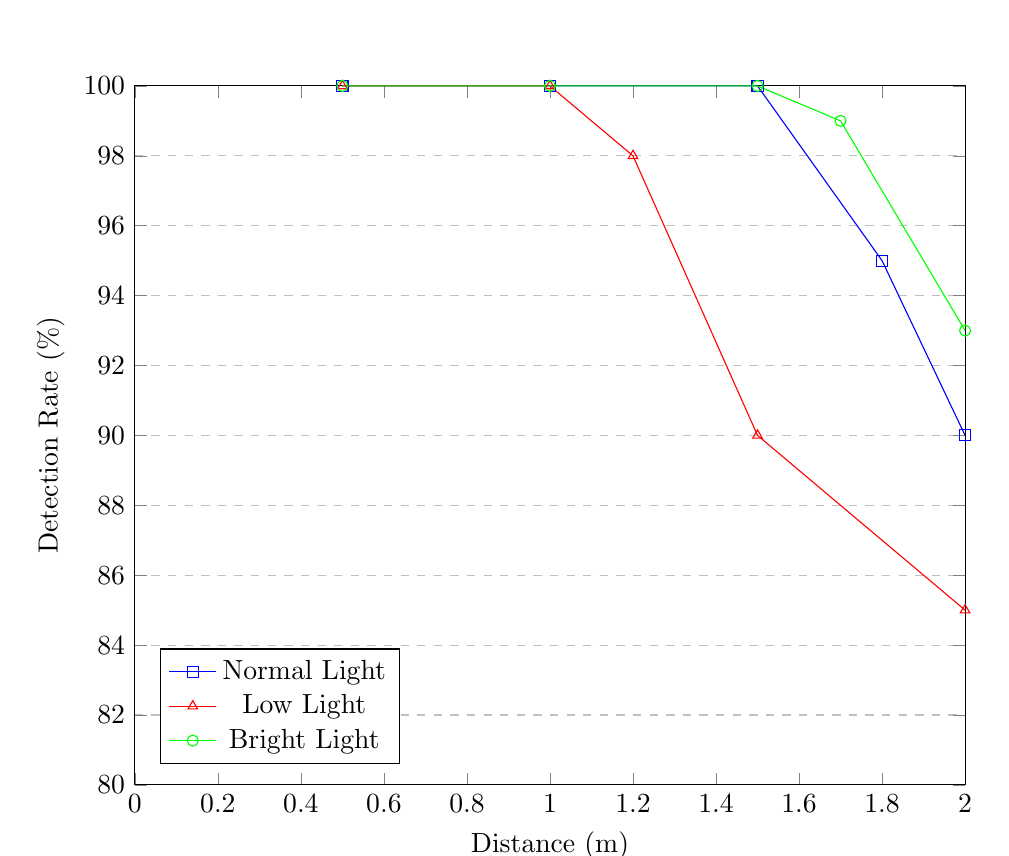
\begin{tikzpicture}[scale=1]  % Slightly scaled down to ensure margin compliance
			\begin{axis}[
				xlabel={Distance (m)},
				ylabel={Detection Rate (\%)},
				xmin=0, xmax=2,
				ymin=80, ymax=100,
				legend pos=south west,
				ymajorgrids=true,
				grid style=dashed,
				width=\textwidth,  % Ensure figure fits within minipage
				]
				
				\addplot[
				color=blue,
				mark=square,
				]
				coordinates {
					(0.5,100)(1.0,100)(1.5,100)(1.8,95)(2.0,90)
				};
				\addlegendentry{Normal Light}
				
				\addplot[
				color=red,
				mark=triangle,
				]
				coordinates {
					(0.5,100)(1.0,100)(1.2,98)(1.5,90)(2.0,85)
				};
				\addlegendentry{Low Light}
				
				\addplot[
				color=green,
				mark=o,
				]
				coordinates {
					(0.5,100)(1.0,100)(1.5,100)(1.7,99)(2.0,93)
				};
				\addlegendentry{Bright Light}
			\end{axis}
		\end{tikzpicture}
		\caption{ArUco Marker Detection Rate vs. Distance}
		\label{fig:detection_rate}
	\end{minipage}%
	\hspace{0.03\textwidth}  % Add explicit horizontal spacing between figures
	\begin{minipage}[t]{0.48\textwidth}
		\centering
		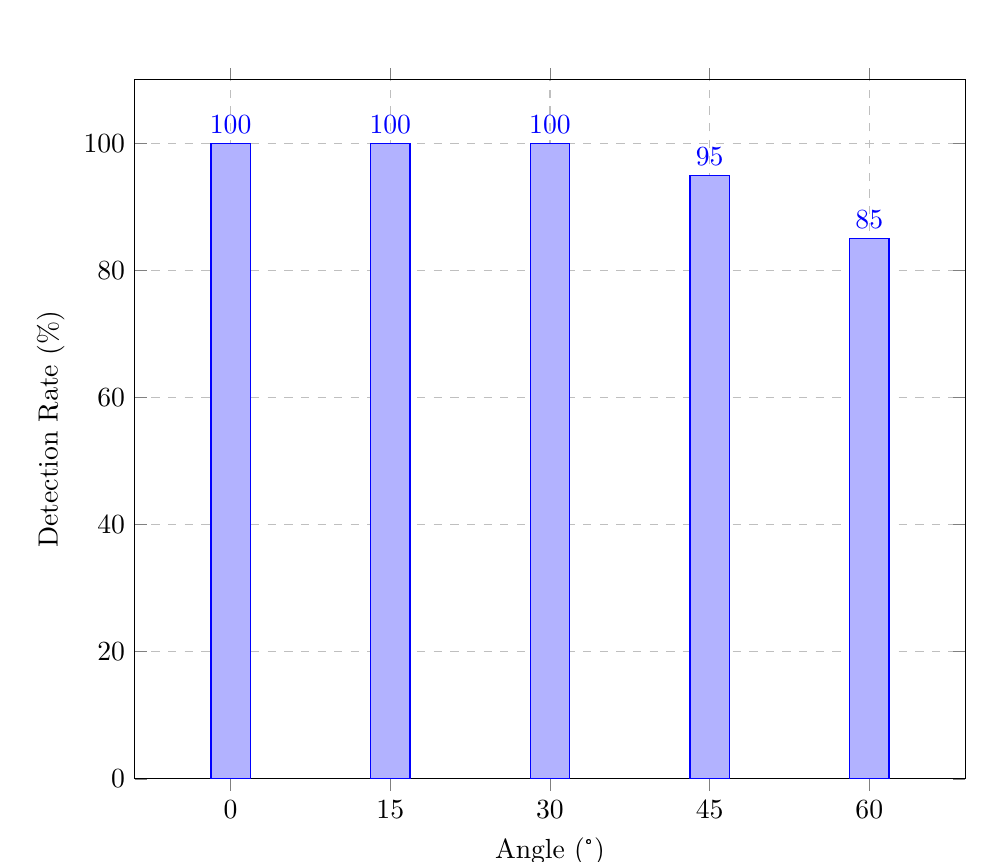
\begin{tikzpicture}[scale=1]  % Slightly scaled down to ensure margin compliance
			\begin{axis}[
				ybar,
				bar width=0.5cm,
				enlarge x limits=0.15,
				ylabel={Detection Rate (\%)},
				xlabel={Angle (°)},
				symbolic x coords={0, 15, 30, 45, 60},
				xtick=data,
				ymin=0, ymax=110,
				nodes near coords,
				grid=major,
				ymajorgrids=true,
				grid style=dashed,
				width=\textwidth  % Ensure figure fits within minipage
				]
				\addplot coordinates {(0,100) (15,100) (30,100) (45,95) (60,85)};
			\end{axis}
		\end{tikzpicture}
		\caption{Detection Rate vs. Angle for ArUco Marker Detection}
		\label{fig:angle_detection}
	\end{minipage}
\end{figure}

\textbf{Angle Robustness:} 
For angular testing, 100 images were captured at angles from 0° to 60° in 15° increments. Detection rates were analyzed to understand performance under different orientations.



\subsubsection{Distance Measurement Testing}
\textbf{Data Collection:} 
Measurements were taken using the \texttt{estimate\_pose} function at fixed distances (0.5m, 1m, 1.5m, 2m), with 100 samples at each point.

\textbf{Analysis:} 
The Mean Absolute Error (MAE) was calculated between measured and actual distances. Consistency was tested by taking 500 consecutive measurements at 1m, calculating standard deviations and confidence intervals.

\begin{table}[H]
	\centering
	\caption{Distance Measurement Accuracy}
	\label{tab:distance_accuracy}
	\begin{tabular}{ccc}
		\hline
		\textbf{Actual Distance} & \textbf{Mean Absolute Error} & \textbf{Error Percentage} \\
		\hline
		0.5m & 0.015m & 3.0\% \\
		1.0m & 0.025m & 2.5\% \\
		1.5m & 0.045m & 3.0\% \\
		2.0m & 0.070m & 3.5\% \\
		\hline
	\end{tabular}
\end{table}


These comprehensive tests validate the ArUco marker detection system's performance, accuracy, and reliability across various conditions. The results demonstrate the system's capability to provide accurate distance measurements and speed estimations, crucial for the robot's navigation and interaction with its environment. The high detection rates and low processing times confirm the suitability of ArUco markers for our real-time robotics application, aligning with the findings of Patru et al. \cite{patru2023empirical}.

The integration testing results confirm that the complete system can operate in real-time, successfully detecting markers, estimating distances and speeds, and responding to control zones. These findings provide a solid foundation for the robot's ability to navigate and interact with its environment using ArUco markers as reference points.





\section{Subsystem Combinations Testing}

After independent testing, the next phase was to combine the subsystems and test their interactions.

\subsection{Camera and Web Interface Integration}

The integration of the camera feed into the web interface was essential for providing real-time visual feedback to the user. The camera was initially connected to the Raspberry Pi, and a Flask-based web interface was used to stream the video feed. The initial implementation focused on setting up the basic functionality of streaming the live video feed through a web page.

\subsubsection{Testing Video Streaming Performance}

Once the camera feed was integrated into the web interface, the system was tested to evaluate its performance. During the initial tests, it was observed that the video stream had a significant lag of \textbf{2-3 seconds}. This was primarily due to the high frame rate of \textbf{30 FPS} (frames per second), which caused data transmission to overwhelm the available bandwidth. The delay resulted in a poor user experience, especially when real-time responsiveness was crucial for controlling the robot.

To assess the performance:
\begin{itemize}
	\item The latency was measured as the delay between the video captured by the camera and its display on the web interface.
	\item The frame rate, resolution, and bandwidth usage were analyzed to determine the cause of the performance bottlenecks.
	\item It was also noted that the web browser’s buffering behavior contributed to the observed lag.
\end{itemize}

\subsubsection{Performance Optimization and Improvements}

To improve the streaming performance, several optimizations were implemented. The following changes were made:

\begin{itemize}
	\item \textbf{Frame Rate Reduction}: The frame rate was reduced from \textbf{60 FPS} to \textbf{30 FPS}. This lowered the amount of data transmitted per second, reducing the load on both the network and the Raspberry Pi, thereby decreasing the lag.
	\item \textbf{Resolution Adjustment}: The resolution of the video feed was scaled down to \textbf{640x480}. This significantly reduced the bandwidth consumption, enabling a smoother video feed without affecting the user's ability to interact with the system effectively.
\end{itemize}

\textbf{Final Results:}
\begin{itemize}
	\item Initial lag: \textbf{2-3 seconds} at 60 FPS.
	\item Optimized lag: \textbf{500ms} at 30 FPS with \textbf{320x240} resolution.
	\item Smooth, reliable video streaming with minimal frame drops.
\end{itemize}

This phase of testing ensured that the camera feed was effectively integrated into the web interface and optimized to provide responsive, real-time feedback necessary for controlling the robot.


\subsection{Web Interface and Motor Control Integration}

For integrating the web interface and motor control, the following steps were taken:

\begin{enumerate}
	\item Developing a separate program to listen for key inputs (W, A, S, D).
	\item Using SocketIO for real-time communication between the web interface and motor control program.
	\item Creating an interface to send PWM signals from the web interface to the motors via the H-bridge.
\end{enumerate}


% Now, include the code:
\begin{lstlisting}[style=pythonstyle, caption=SocketIO event handler for robot movement]
	# SocketIO event to handle robot movement
	@socketio.on('move')
	def handle_move(direction):
		global forward_disabled
		if direction == 'forward' and forward_disabled:
			print("Forward movement is disabled [restricted zone]")
			robot.stop()
		elif direction == 'forward':
			robot.move_forward()
		elif direction == 'backward':
			robot.move_backward()
		elif direction == 'left':
			robot.turn_left()
		elif direction == 'right':
			robot.turn_right()
		elif direction == 'stop':
			robot.stop()
\end{lstlisting}



The web interface successfully controlled the robot's movements, with a measured control latency of \textbf{300ms}. Minor delays were noted during rapid direction changes, which could require further optimization.

\textbf{Results:}
\begin{itemize}
	\item Control latency: \textbf{300ms}.
	\item Issues: Slight delay during rapid changes.
\end{itemize}

\subsection{Web Interface and ArUco Detection Integration}

To integrate ArUco marker detection into the web interface, the camera feed was processed in real time, and marker IDs were displayed on the interface. The system could detect markers with a delay of \textbf{100ms} when more than three markers were present in the frame simultaneously.

\textbf{Results:}
\begin{itemize}
	\item Detection delay: \textbf{100ms} with three or more markers.
	\item Detection accuracy: \textbf{100\%} for up to three markers.
\end{itemize}

\section{Integration Phase}

The final integration phase brought together the core components: \textbf{Aruco marker detection}, \textbf{motor control}, and the \textbf{web interface}. This stage focused on combining the previously tested individual systems into a unified framework capable of real-time robot control and marker detection.

Key steps included:
\begin{enumerate}
	\item Merging the motor control program with the ArUco marker detection system to allow the robot to respond to detected markers.
	\item Real-time processing of the video feed from the camera for marker detection, alongside real-time control through the web interface.
	\item Implementing pre-defined behaviors that adjusted motor actions (such as speed and direction changes) based on the specific markers detected by the camera.
\end{enumerate}

Features such as distance measurement, speed estimation, and marker-based tasks were also developed and tested independently before being added to the full system. These functionalities were integrated step-by-step to ensure proper interaction between components.

A more detailed discussion of the final system’s performance, including its compliance with the Acceptance Test Procedures (ATPs), will be covered in the next chapter. There, the results of the fully integrated system will be examined in line with the project's objectives.

%@@@@@@ Chapter 5 - Results and Discussion @@@@@@@@@@@@@@@@@@@@@@@@@@@@@@@@@@@@@@
\chapter{\label{ch:results} Results and Discussion}

This chapter describes the tests that were carried out in order to test the system to see that it works according to specified user requirements in section. The system under test was designed in Chapter~\ref{ch:ch4}.

\section{\label{sec:ch5_subsec1}Subsection Name}

This section describes some results. This is how you can reference an appendix Appendix~\ref{app:sec:myappendix} as you might want to offload stuff to the appendix.

Here is an example table

\begin{table}[!ht]
	\centering
	\caption{Caption for table}
	\begin{tabular}{l|l}
		\hline
		\textbf{Parameter}      & \textbf{Value}   \\ \hline
		Lower cutoff frequency  & 100 kHz  \\
		Mid frequency           & 200 kHz \\
		Higher cutoff frequency & 300 kHz \\ \hline
	\end{tabular}
	\label{tb:mytablename}
\end{table}


%@@@@@@ Chapter 6 - Conclusions and Further Work @@@@@@@@@@@@@@@@@@@@@@@@@@@@@@@@
\chapter{\label{ch:conclusions} Conclusions and Further Work}

This chapter presents the conclusions and future work for this dissertation.

\section{Conclusions}

\begin{figure}[!ht]
	\centering
	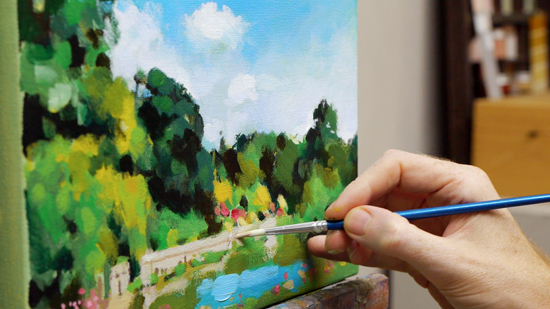
\includegraphics[width=1.0\textwidth]{ch6/figs/picture.jpg}
	\caption{Useful concluding diagram}
	\label{fig:picture1}
\end{figure}

\section{Recommendations For Further Work}





%@@@@@@@@@@@@@@@@@@@@@@@@@@@@@@@@@@@@@@@@@@@@@@@@@@@@@@@@@@@@@@@@@@@@
%@@@@@@@@@@@@@@@@@ References @@@@@@@@@@@@@@@@@@@@@@@@@@@@@@@@@@@@@@@
%=============================
\bibliography{bibliography}

%=============================
\appendix

%\newpage
%%@@@@@@@@@@@@@@@@@@@@@@@@@@@@@@@@@@@@@@@@@@@@@@@@@@@@@@@@@@@@@@@@@@@@@@@@@@@@@@@@@
%%@@@@@@@@@@@@@@@@@@@@@ APPENDIX @@@@@@@@@@@@@@@@@@@@@@@@@@@@@@@@@@@@@@@@@@@@@@@@@@
%%@@@@@@@@@@@@@@@@@@@@@@@@@@@@@@@@@@@@@@@@@@@@@@@@@@@@@@@@@@@@@@@@@@@@@@@@@@@@@@@@@

\chapter{\label{app:myappendix}ADC/DAC core}

\section{\label{app:sec:myappendix}A useful sub appendix}

Put your appendix stuff here.


\end{document}
